\documentclass[11pt]{article}
%Gummi|063|=)
\title{\textbf{The fabrik of knowledge}}
\usepackage{graphicx}
\usepackage{amsmath}
\begin{document}
\maketitle


\section{smallest part of what we call knowledge}
The picture shows an assemblage of concepts as they look when plotted with GraphViz.
Its a bit like snow as every concept has a different structure,
some simple ones some complex generally a concept can have one ore more 
exits which lead into one or more related concepts like\\
( I'm going = to the shop // crazy )

using graph wizard for sampling concepts one level only!!!


\begin{figure}[htp]
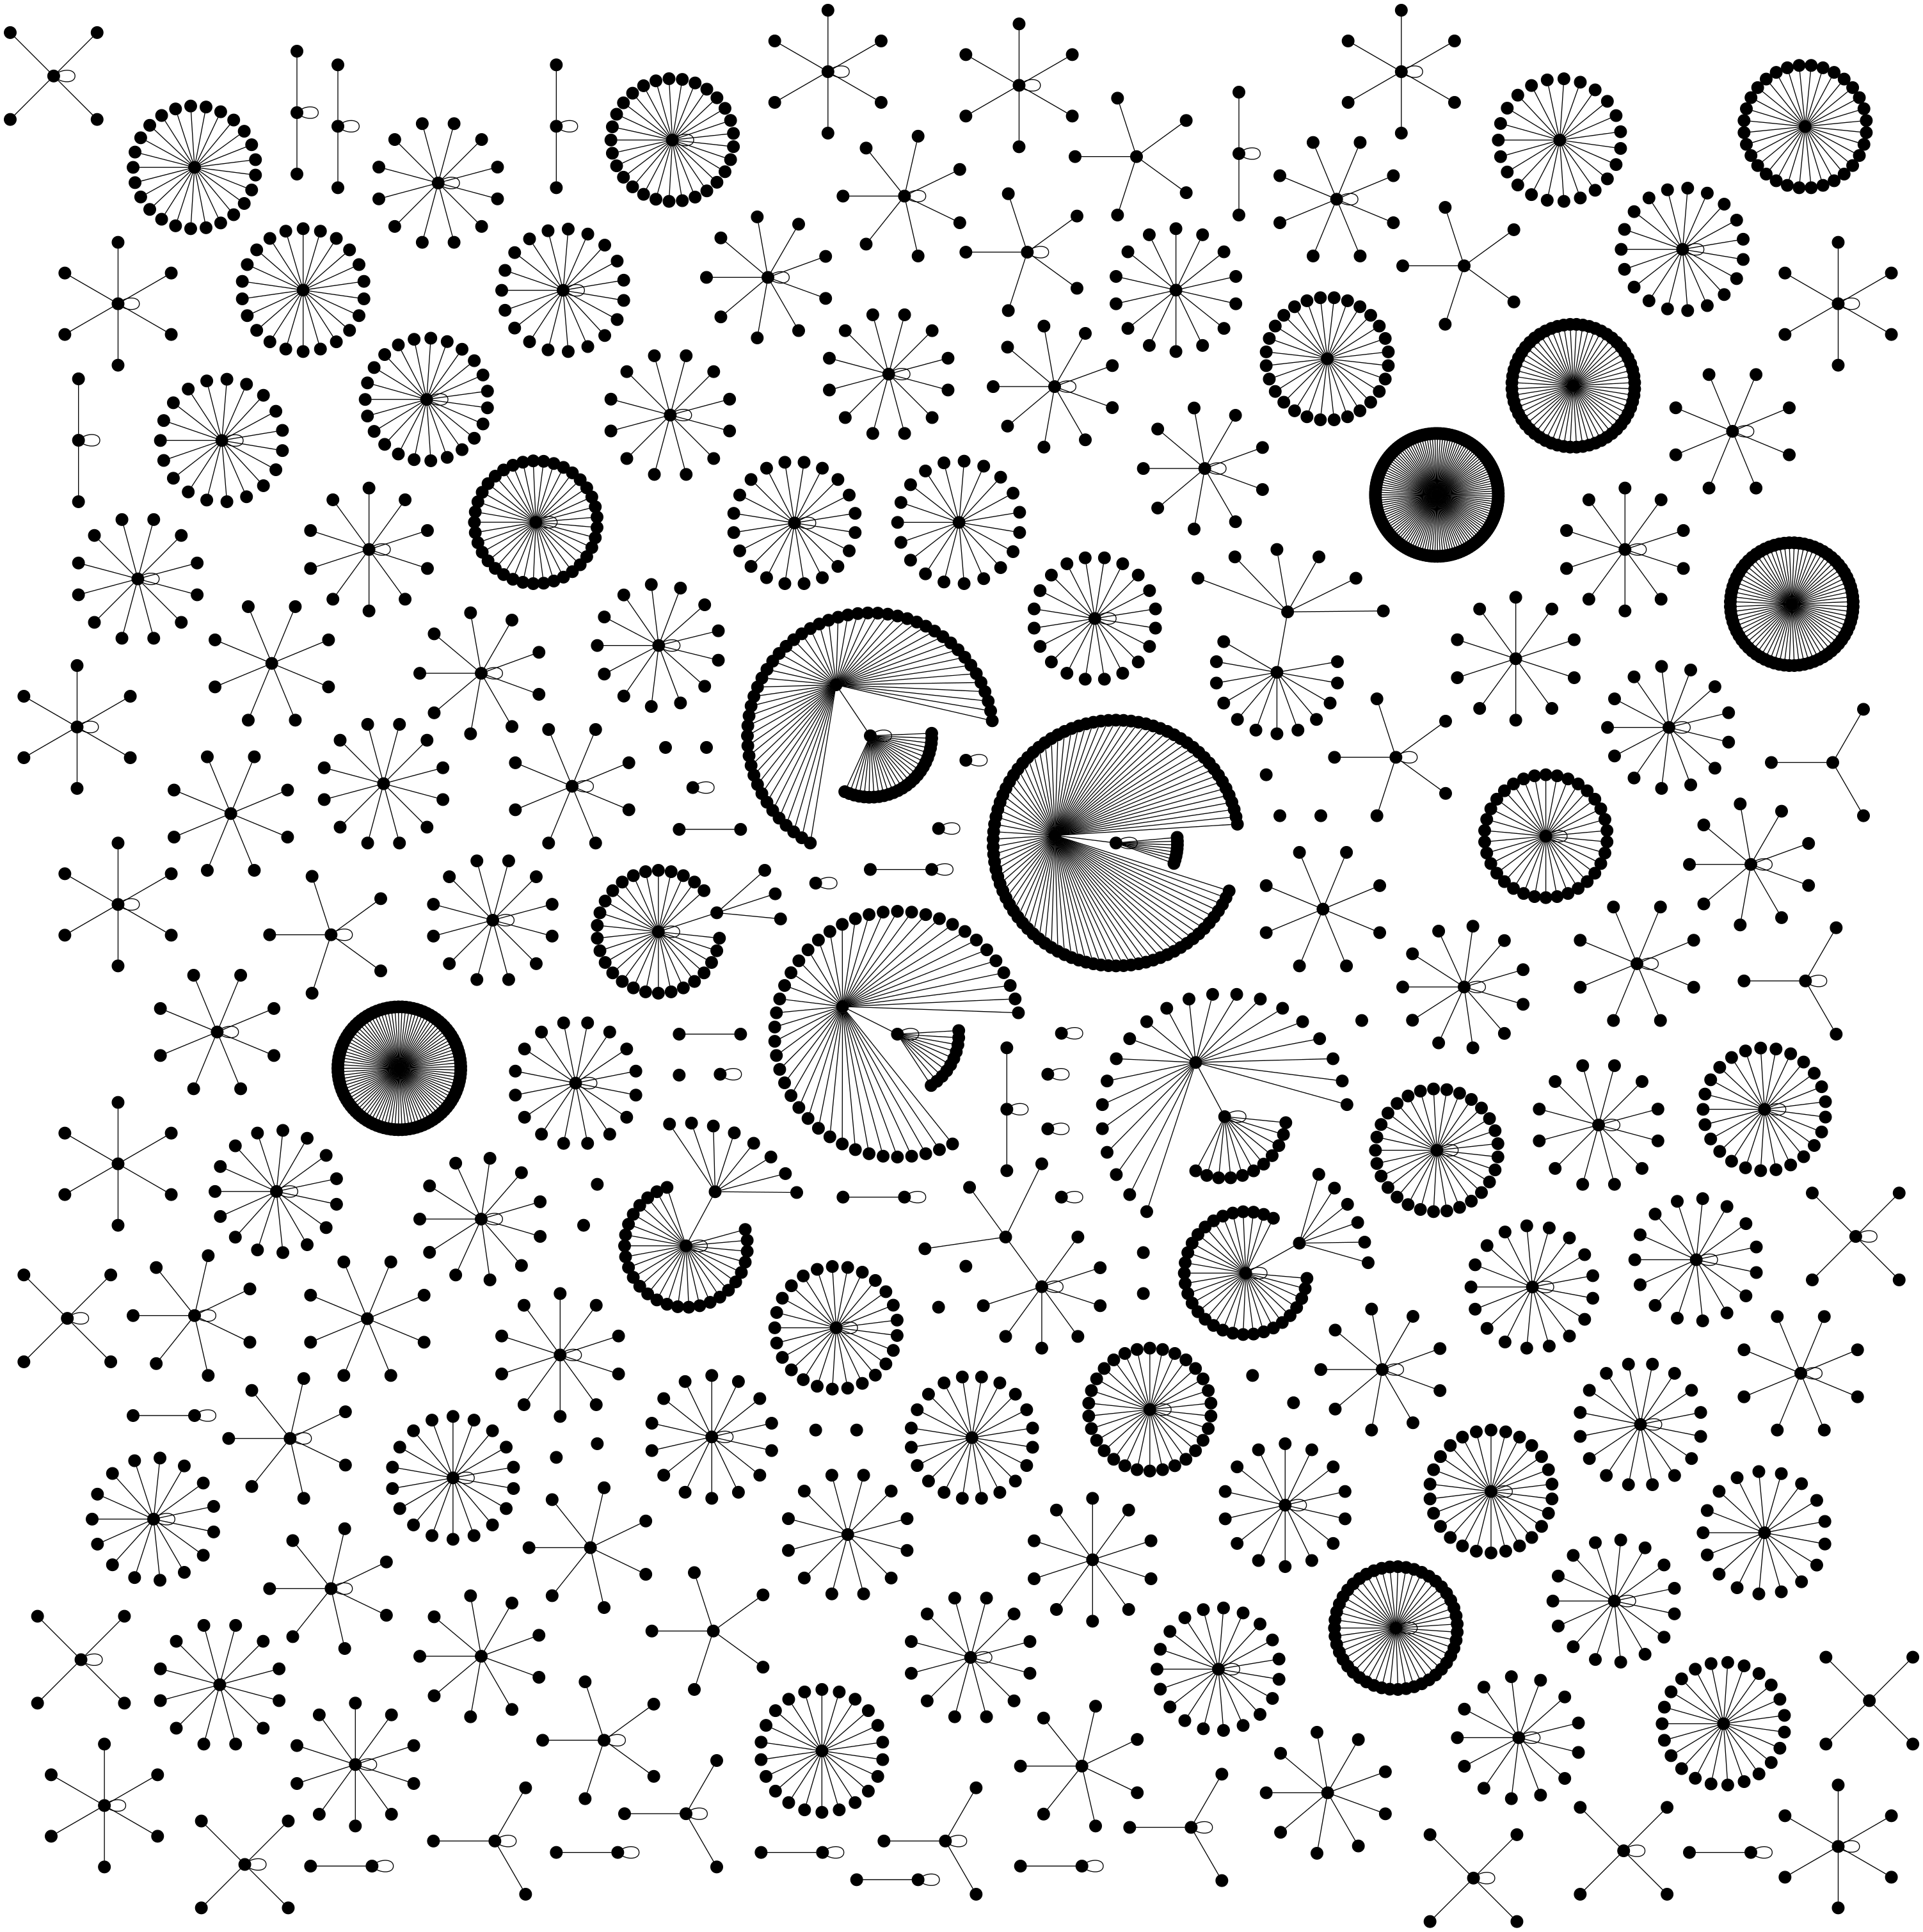
\includegraphics[scale=0.14]{img/a_directories.png}
\caption{generating fairly random concepts with common letter [a] }
\label{}
\end{figure}



\begin{figure}[htp]
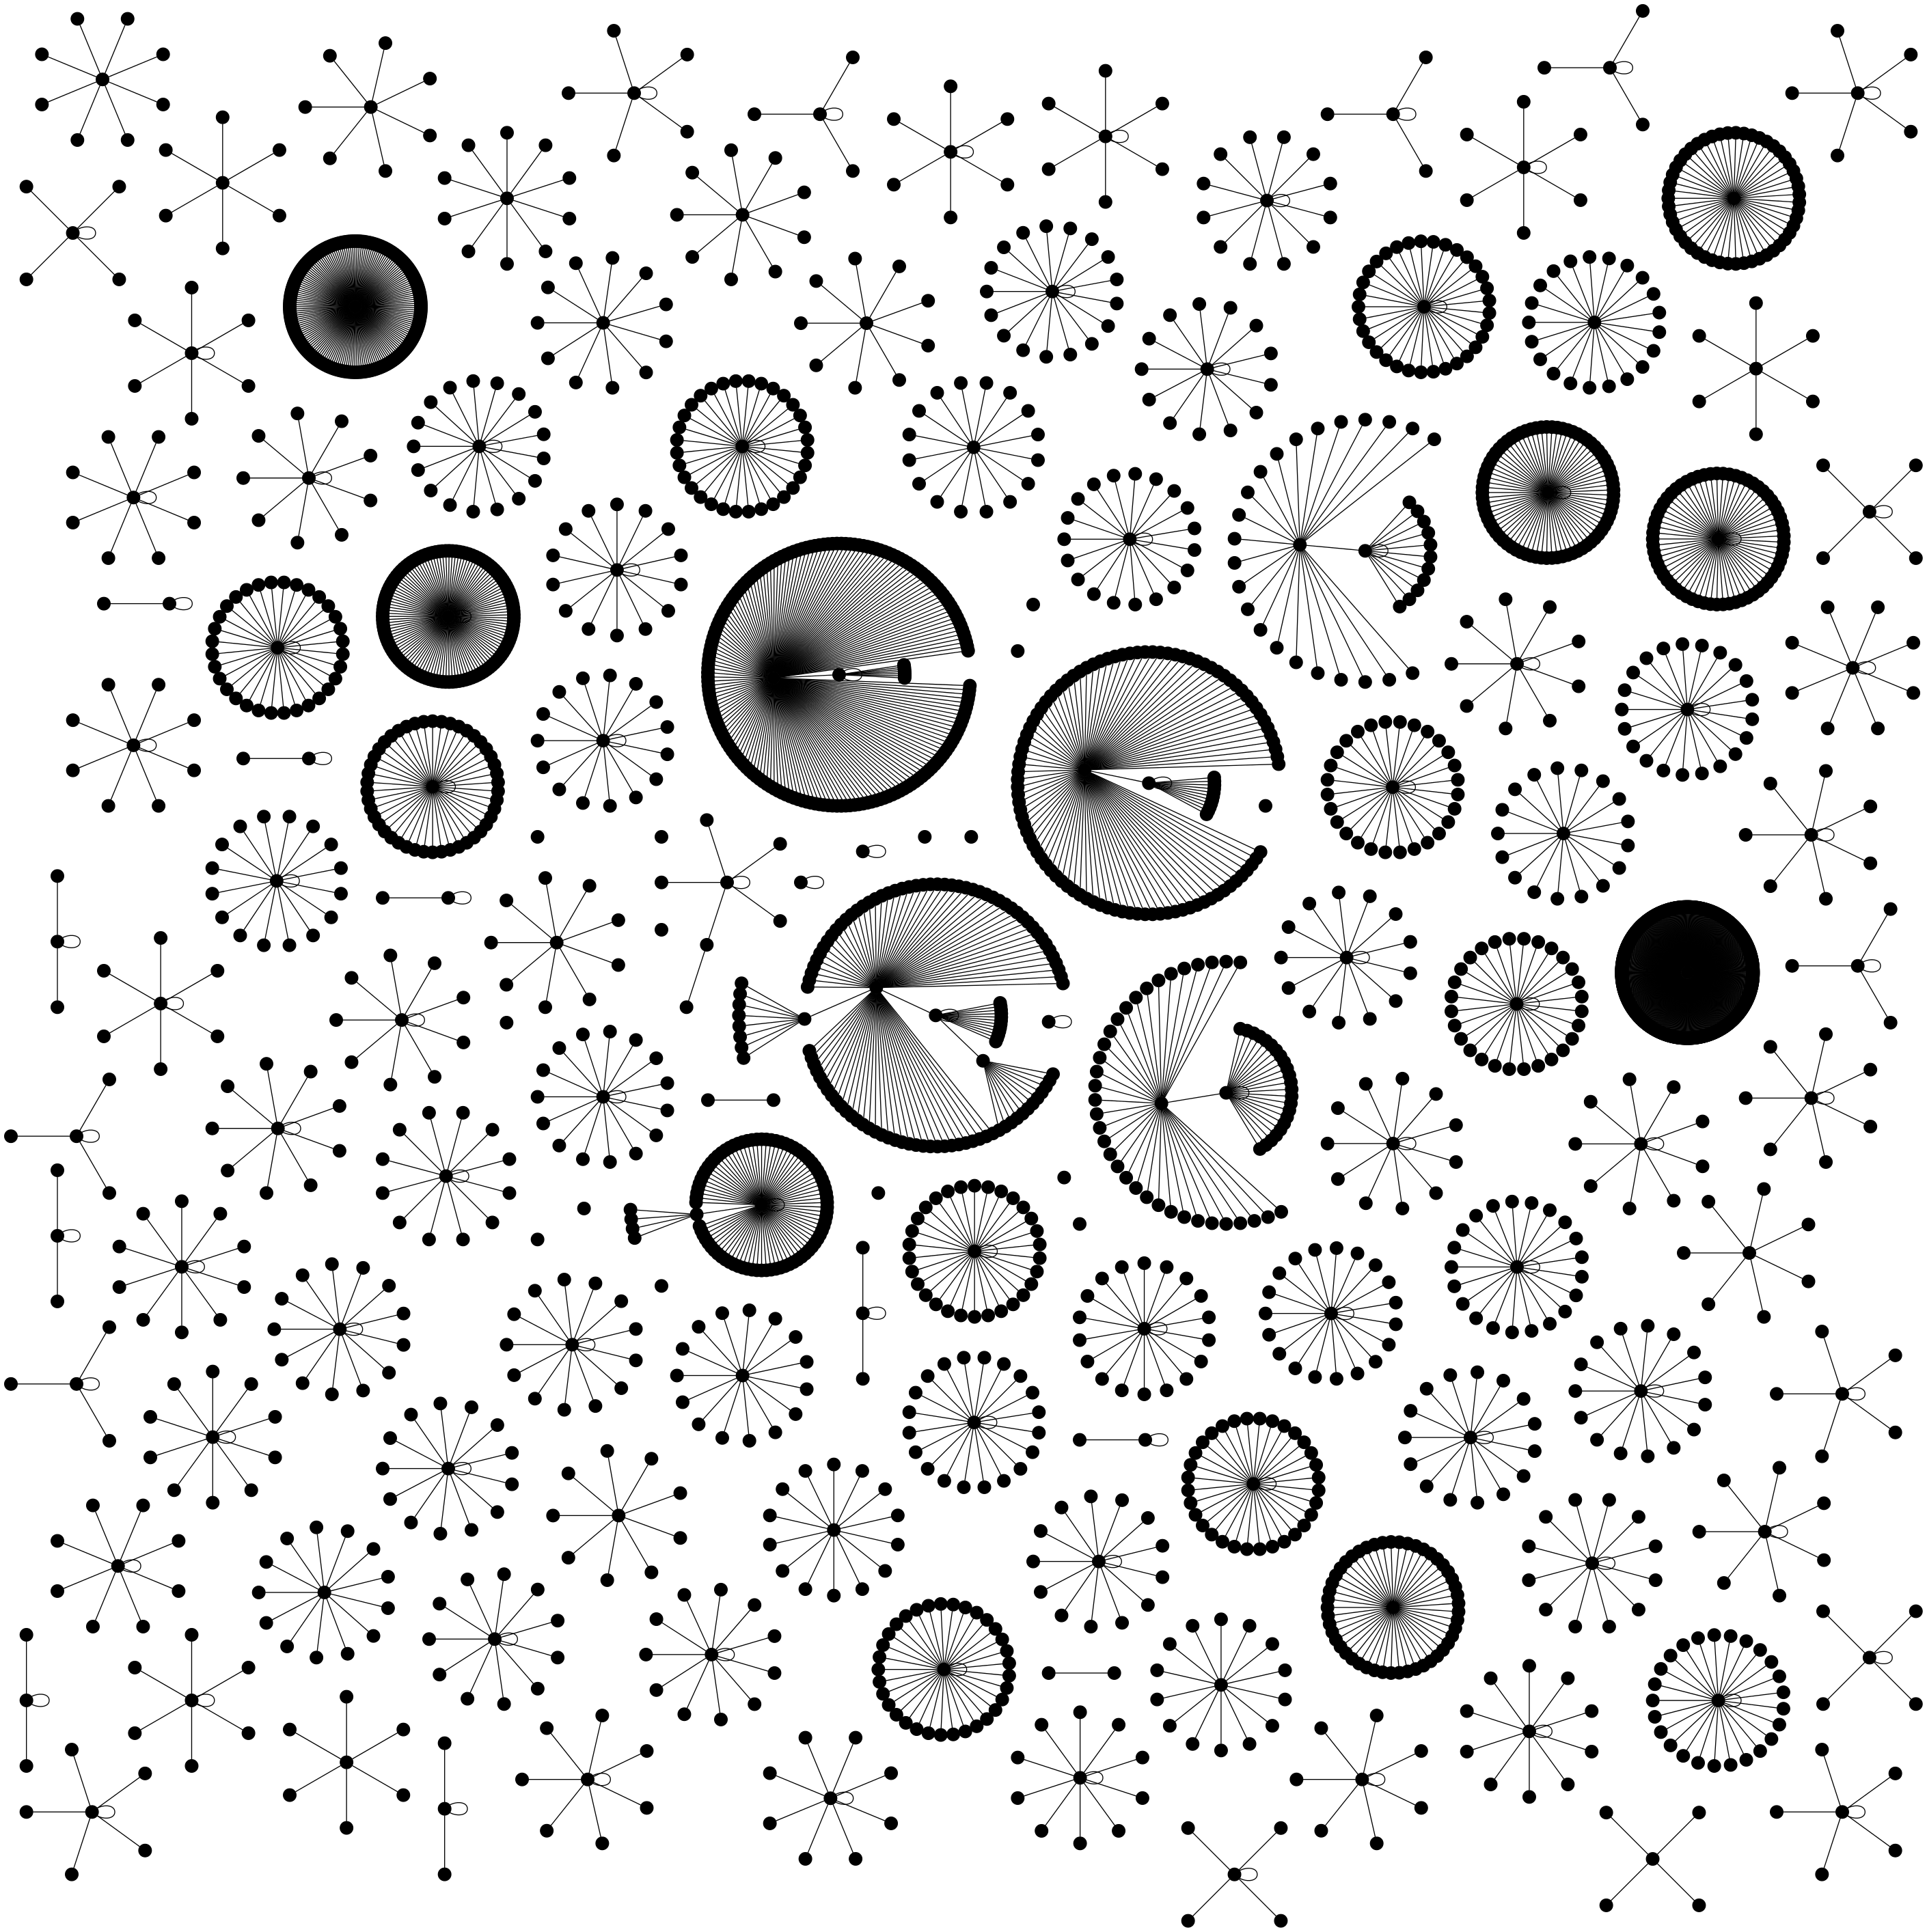
\includegraphics[scale=0.14]{img/m_directories.png}
\caption{a random generation of unrelated concepts}
\label{}
\end{figure}




common character [w]

\begin{figure}[htp]
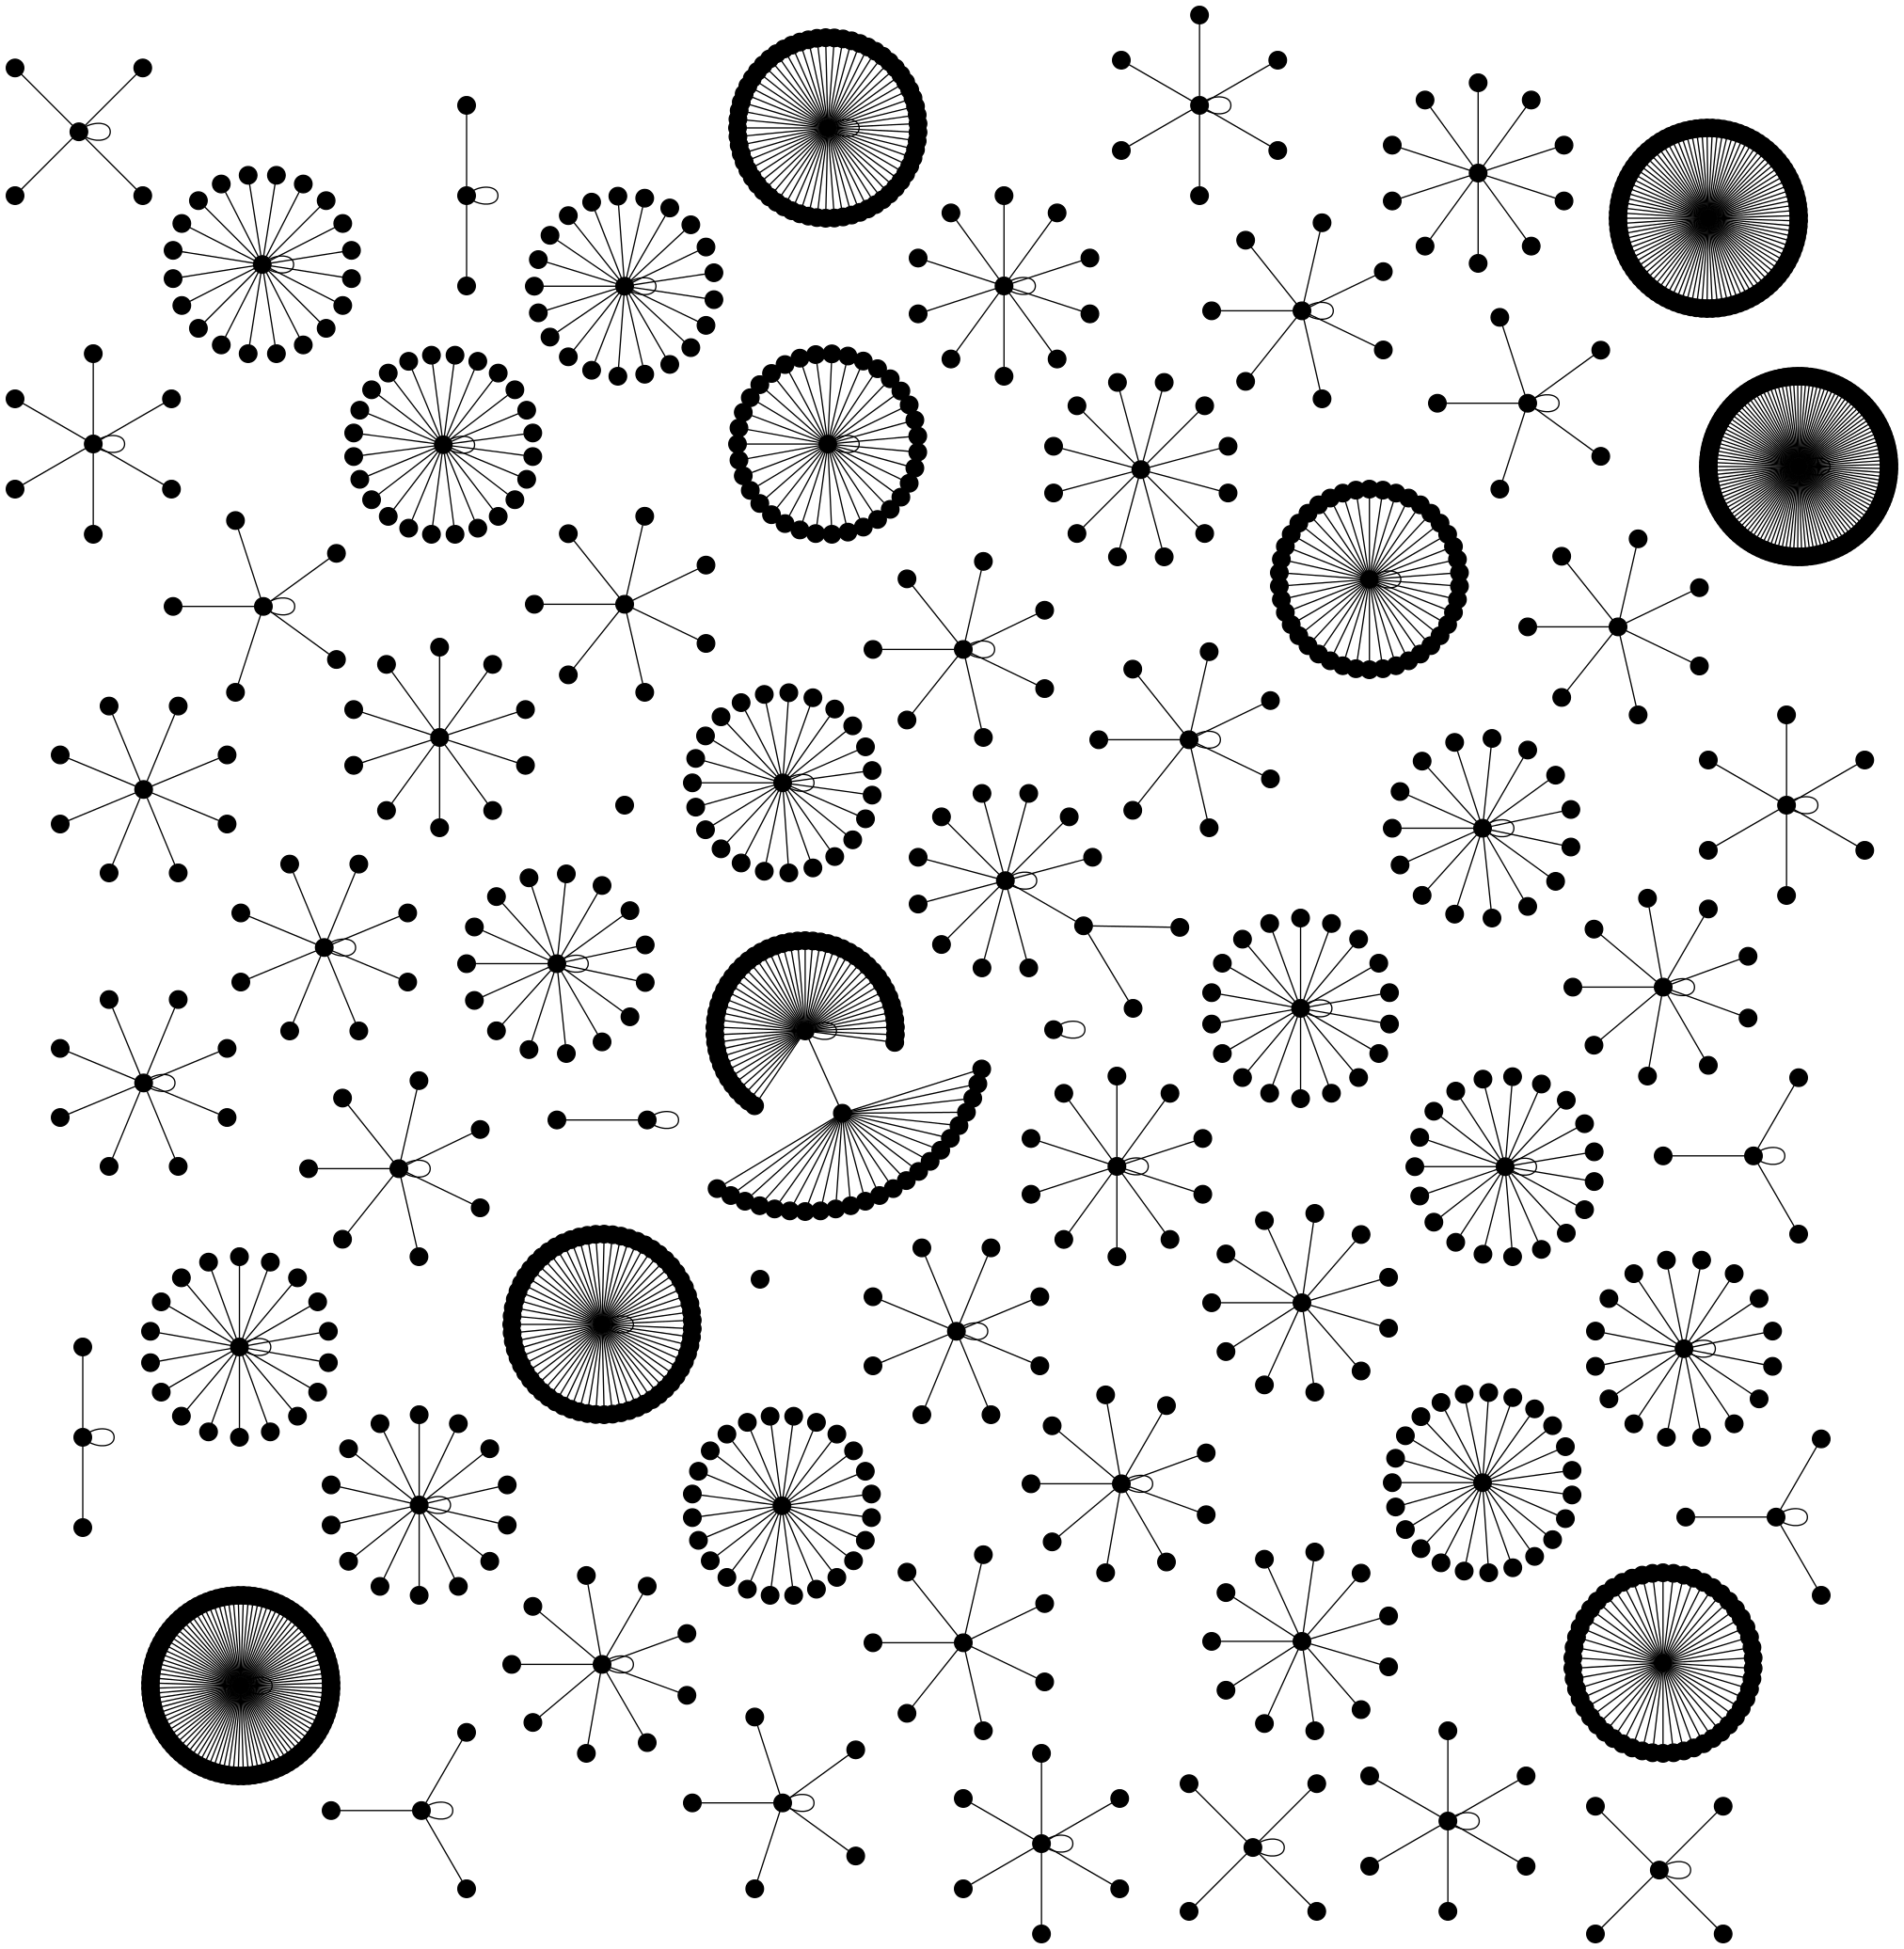
\includegraphics[scale=0.20]{img/w_directories.png}
\caption{a random generation of unrelated concepts}
\label{}
\end{figure}




\section{A knowledge system }

A large number of concepts even if assembled randomly 
will form a system where the relations will form connections 
which would make it possible to move from one concept to any other within 
the system.

\begin{figure}[htp]
\centering
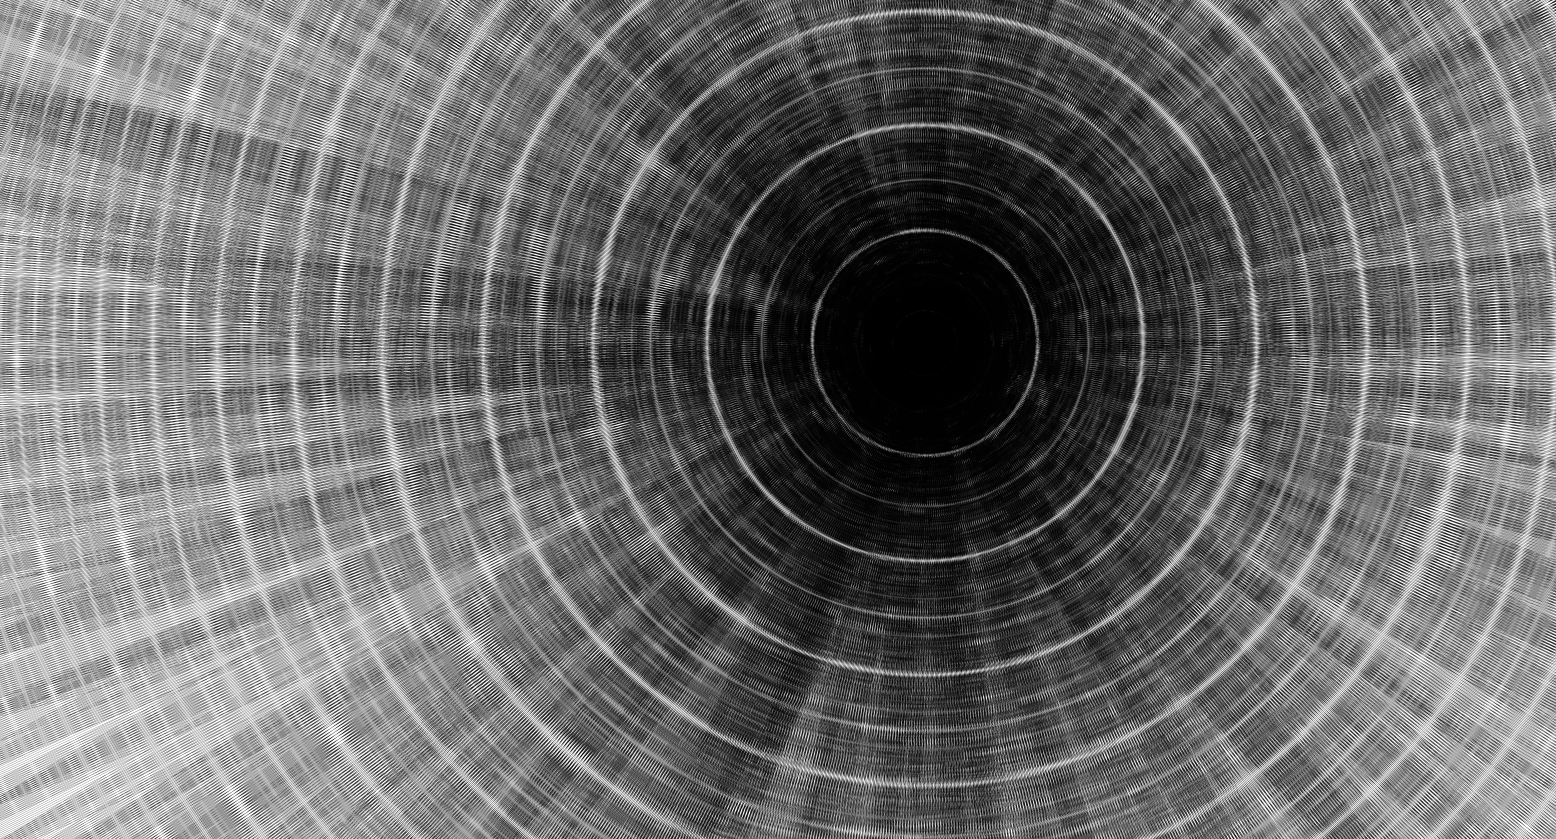
\includegraphics[scale=0.40]{img/1362924302_directories.png}
\caption{knowledge system with round about 1k concepts}
\label{every thought is interlocked somewhere at some point}
\end{figure}



\section{Making knowledge}
Lets start to render something simple like 
science-fiction


\begin{figure}[htp]
\centering
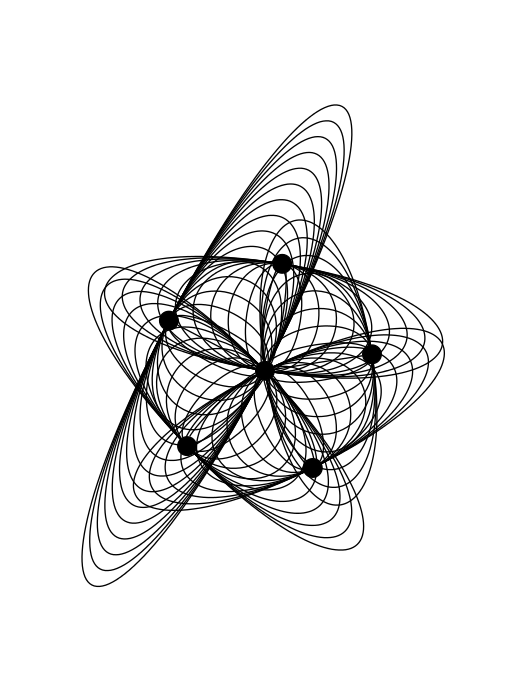
\includegraphics[scale=0.80]{img/science_fiction_directories.png}
\caption{}
\label{}
\end{figure}


\begin{tabular}{lllllllllll}
	11 & 12 & 13 & 14 & 15 & 16 & 17 & 18 & 19 & 110 & 111\\
	21 & 22 & 23 & 24 & 25 & 26 & 27 & 28 & 29 & 210 & 211\\
	31 & 32 & 33 & 34 & 35 & 36 & 37 & 38 & 39 & 310 & 311\\
	41 & 42 & 43 & 44 & 45 & 46 & 47 & 48 & 49 & 410 & 411\\
	51 & 52 & 53 & 54 & 55 & 56 & 57 & 58 & 59 & 510 & 511\\
\end{tabular}


\begin{figure}[htp]
\centering
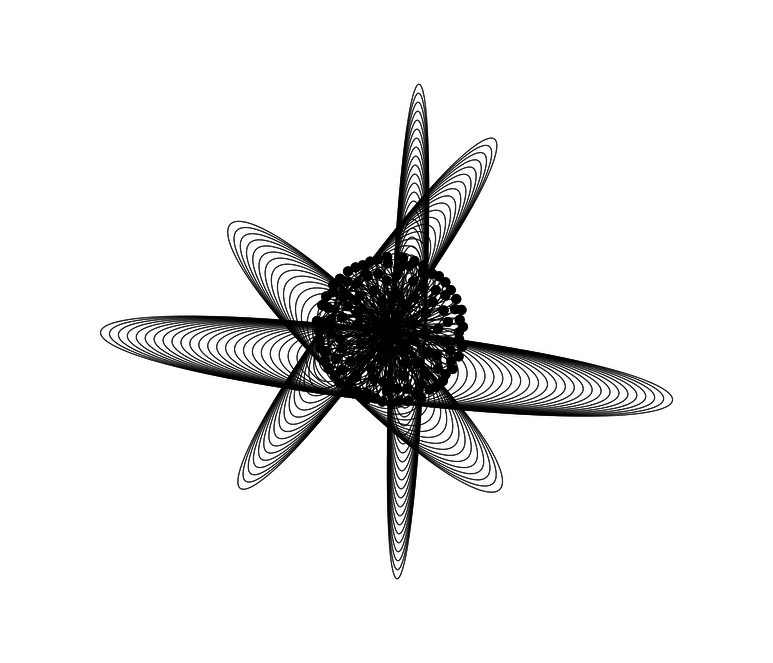
\includegraphics[scale=0.6]{1363498617__knowledge-reactor.png}
\caption{}
\label{}
\end{figure}

\end{document}

